\definecolor{light-gray}{gray}{0.95}
\lstset{basicstyle=\ttfamily\footnotesize,
    backgroundcolor=\color{light-gray}, xleftmargin=0.7cm,
    frame=tlbr, framesep=0.2cm, framerule=0pt,
}

\section{Introduction}

%The \textit{proceedings} are the records of a conference.\footnote{This
%  is a footnote}  
With the advent of technology there has been a rapid increase in the use of low power embedded devices. These devices are deployed in wide and diverse applications, and are connected to the internet. With these devices becoming more pervasive, large scale attacks involving compromised embedded devices such as the Mirai botnet are becoming commonplace. In absence of robust secure environment, vulnerabilities introduced in these devices due to programming flaws can allow attackers to take control with ease.\\

Several of these vulnerabilities occur due to illegal use of memory accesses. In spite of having memory safe languages like Java, Python and C\#, most of these vulnerabilities still persists because even today operating system, virtual machine monitors, embedded systems, database management software's, web browsers are developed in C/C++. The sole purpose of this being these languages provide low level memory management support and allow explicit manual memory management and are very close to the hardware. However these allowance of explicit memory management feature comes up with a price of illegal memory access and has lead to many attacks in the past. Now replacing all of the existing code in memory safe languages is not a feasible option as it's not a cost effective solution and hence we are left with a difficult task of retrofitting security in the existing system. Even in today's world these memory access vulnerabilities still rank among the top 25 vulnerabilities in system software\cite{Top25} and vulnerabilities like buffer overflows\cite{Aleph}, Use-After-Free(UAF)\cite{NIST,DataAttacks,BeyondStackSmashing} double free are one of the major reasons for causing security threats and crashing down systems.\\

In the past there has been many studies relating to spatial and temporal attacks \cite{BaggyBounds, Valgrind,CCured,SoftBound,Mudflap,BackwardChecking,LLP,DFI,DieHard,Austin,CETS,Fischer,ComprehesiveMemsafety,Watchdog,Hardbound,AccMetaDataChecks,IGPM} and there also have been several proposals to prevent one or both of these attacks. Some of these solutions focused only on software tools \cite{BaggyBounds, Valgrind,CCured,SoftBound,Mudflap,BackwardChecking,LLP,DFI,DieHard,Austin,CETS} whereas some solutions relied upon the hardware \cite{Fischer,ComprehesiveMemsafety,Watchdog,Hardbound,AccMetaDataChecks,IGPM}, to enforce security. But most of the software solutions[citations required ] either fails to provide complete temporal and spatial safety or they just incur too much run time overheads. Purely software solutions like \cite{SoftBound} and \cite{CETS} both combined tackle all possible kinds of spatial and temporal attacks but has high code size and runtime overheads. Whereas on the other hand hardware solutions like \cite{Shakti-T,Watchdog} may reduce the run time overhead but on the contrary introduces hardware complexities and require additional data structures to maintain pointer metadata. Shakti-T\cite{Shakti-T} provides complete memory safety(temporal and spatial) but being only a hardware solution requires specialized hardware to perform, i.e. it uses a separate BnBCache to store pointer metadata. On the other hand Watchdog\cite{Watchdog} in-spite of being a compiler plus hardware solution it uses shadow space to maintain the pointer id's, base and bounds and uses CPU-inserted Micro-Ops to validate memory operations. So Watchdog also requires  specialized hardware to maintain the pointer metadata and it has a high overhead of shadow memory i.e nearly 3/4 of the memory is inaccessible. Moreover Gandalf\cite{Gandlaf} seems to have a hardware plus solution without any extra hardware complexity and minimal compiler modifications. However, it does not provide temporal safety, and requires modifications to be made to the operating system.\\

In this paper, we propose a complete memory safety solution(both temporal and spatial) by making modifications in the compiler to insert certain operations in parts of the generated machine code and make small additions to the hardware to accelerate these operations. Moreover we are not using any separate region of memory like shadow space or metadata tables, which in turn reduces the hardware complexities and storage overhead. In our approach to prevent spatial and temporal attacks on stacks, each pointer is associated with a base, bound and id\_hash (each 32 bits wide) which is stored as a 128-bit "fat pointer" on the stack. Every use of the pointer validates the base and bound, matches the id\_hash with the hash computed from the stack frame cookie as described in \ref{terms}.\ref{SFC} and then performs the required operation.  The storage overhead is an additional 96 bits per pointer and 64 bits per stack frame, which is at par, if not better than existing solutions. Similarly to ensure spatial and temporal safety on heap allocated memory, each malloc chunk will now be associated with a 64-bit random number to help craft a 128-bit pointer object consisting of base bound id\_hash and the pointer itself. Every use of the pointer will have validity checks inserted before them by the compiler. The memory overhead for n pointers pointing to a single malloc chunk is 96*n + 64. The worst case memory overhead to prevent both spatial and temporal attacks in stack and heap with n pointers to heap/variables on stack and m malloc chunks/stack frames would be 128*n + 64*m . The insertion of fat pointers and validity checks has been implemented through a transformation pass in RISCV-LLVM. THe transformation pass operates on the intermediate representation generated by the compiler frontend before passing it to the compiler backed for machine code generation. The hardware was developed in Bluespec-System-Verilog\cite{Bluespec} as an extension to the SHAKTI class of RISCV processors developed at RISE lab.\\

The remainder of the paper is organized as follows: Section 2 describes some of the terminologies used in \ref{name}. It also describes the proposed plan to prevent temporal and spatial attacks on stacks and heaps. Section 3 describes the details of the compiler modification required for \ref{name}, and the Microarchitectural implementations of \ref{name}. Section 4 presents some of the case studies demonstrating how the compiler modifications and the hardware work to prevent certain attack scenarios. Section 5 deals with some of the analysis and  result of \ref{name}. Section 6 concludes the paper.

\begin{figure}
\centering
\captionsetup{justification=centering}
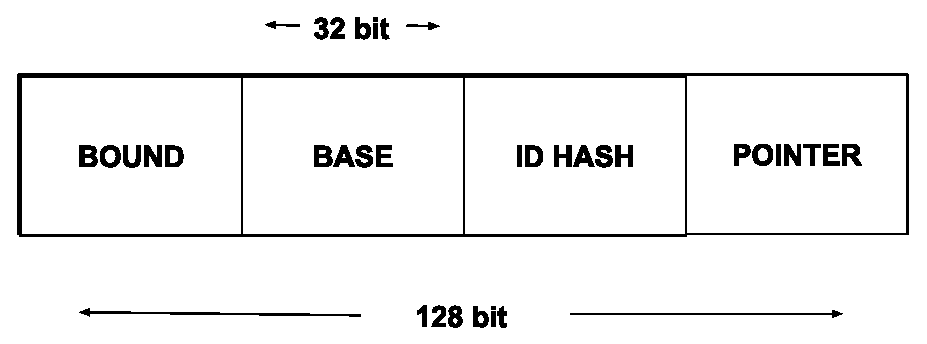
\includegraphics[width=8cm]{fat_pointer.eps}
\caption{Structure of metadata in Fat pointer}
\label{fig: metadata}
\hrulefill
\end{figure}

\section{The proposed plan \ref{name}}
In this section we describe certain new terminologies that we have used and then present an abstract overview of how \ref{name} works to provide complete temporal and spatial safety. 
\subsection{Terminologies}\label{terms}
\begin{enumerate}
    \item \textbf{Stack Frame Cookie (SFC)}\label{SFC} : It is a unique 64-bit random number that is placed on the stack frame below all the variables of the current function. This SFC is unique for each function calls and is used to compute the id\_hash of all variables or object available within the scope of that function. Moreover the SFC is dismissed or collapsed once the function goes out of scope ensuring all pointers to be invalid once the function returns.
    \item \textbf{ROData Cookie (RODC)} : It is also a 64-bit unique random number but unless like SFC it is placed on the .bss region of the memory. It is used to protect the read only region of memory to prevent any kind of over-reads or invalid pointer access. The RODC is used to compute id\_hash's of global variables and provide memory safety.
    \item \textbf{ID\_HASH} : It is a 32-bit unsigned number which is computed either from the SFC or RODC or from the unique 64-bit number that is stored along with the malloc chunck. It is also one of the four fields of the fat pointer and the value of ID\_HASH is computed with the help of the new instruction named \textbf{"hash"}(described in section \ref{ISA}.\ref{hash}).
    \item \textbf{BASE} : It is a 32-bit value indicating the base address of the SFC or the RODC or the base of the malloc chunk. It is also one of the fields of the fatpointer and is used or checking the lower bounds.
    \item \textbf{BOUND} : It is a 32-bit value indicating the absolute bound of the object. It is the maximum premissible range that the pointer can point to. 
    \item \textbf{Safe Malloc}\label{safemalloc} : The call to "safemalloc" is similar to malloc expect that it now allocates 8 more bytes than the required malloc chunk as shown in Fig \ref{fig:malloc_chuck} and returns an i128 object. In this extra 8 bytes we store a unique 64 bit random number which acts similarly to the SFC. Now every pointer pointing to this allocated chunk will use this unique 64-bit random number to craft a fat pointer out of it as shown in Fig \ref{fig: metadata}.
    \item \textbf{Safe free} \label{safefree}: The call to "safefree" is similar to free method call but now safefree accepts fat pointers instead of normal pointers. The method safefree first validates the fat pointer and on successful validation calls free internally to deallocate the required region of memory. The method also randomises the 64-bit random number stored along with the malloc chunk, so that any further reference to that region would result in an invalid check.
    \item \textbf{Craft} : It is a method which is used for crafting fat pointers. It accepts four 32-bit number i.e base, bound, id\_hash, and the object itself and then returns an i128 object by creating the fat pointer. Fig \ref{fig: metadata} shows the structure of the fat pointer returned by craft function call.
\end{enumerate}

\begin{figure}
\centering
\captionsetup{justification=centering}
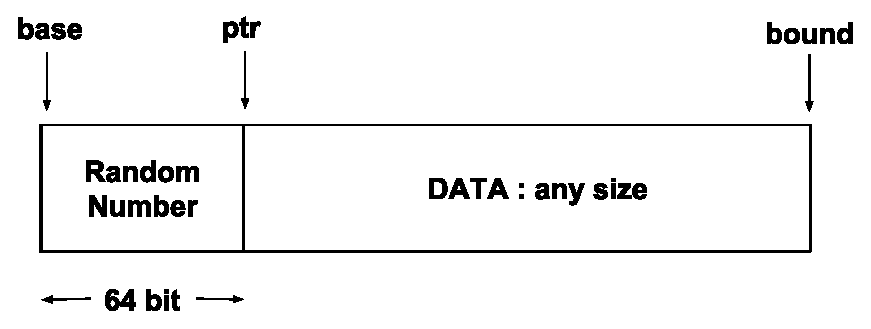
\includegraphics[width=8cm]{malloc.eps}
\caption{Storage of Metadata with along with malloc chunk}
\label{fig:malloc_chuck}
\hrulefill
\end{figure}

\subsection{Preventing Temporal and Spatial attacks on Heaps}

\subsubsection{Preventing Temporal Attacks} :\label{temp_heap}
In the past there has been many ways to prevent against temporal attacks \cite{Austin,DieHard,Dhurjati,Dhurjati1,Purify,Valgrind,Exterminator,Fischer,MemTracker,BackCompTrans,CETS}, most of which can be classified into two categories i.e. location based or an identifier based. The location based\cite{Purify,BackBoundsChecking,Valgrind,MemTracker} approach uses an extra data structure namely a tree or a shadow space to keep track of the allocated and deallocated memory chunk. This method however prevents most uses of dangling pointers but it fails to prevent against pointers where reallocation of memory is used, as it uses the object's address to determine it is allocated or not. On the other hand the identifier based\cite{CETS,Fischer,BackCompTrans} approach uses a per pointer metadata or a lock and key mechanism to prevent against dangling pointers.

In \ref{name} we will be using a mechanism which is similar to lock and key to prevent all kinds of temporal attacks. We know that the basic functions that allow low level  memory management support in C are malloc and free. So in our approach to prevent against dangling pointers and invalid free's we have done slight modifications to these function calls and replaced malloc with "safemalloc"(described in Section \ref{terms}.\ref{safemalloc}) and free with "safefree"(described in Section \ref{terms}.\ref{safefree}) respectively. Now every pointer pointing to that allocated chunk will use the 64-bit random value associated with it to craft a fat pointer. Hence each pointer now has been transformed to a fat pointer and has its own base, bound and id\_hash. Therefore all subsequent loads and stores are validated first and performed on successful validations. Moreover safefree would randomise the 64-bit value stored along with the allocated chunk which further ensures that any reference to that allocated chunk by any pointer would result in a validate error. Moreover the other method which might cause a problem for memory management support is realloc. Now to ensure safer handling of realloc's we have our own "saferealloc" method which replaces all realloc calls in the program. The saferealloc accepts a i128 object and the new modified size as parameters and then performs certain validity checks. The safereaclloc method internally calls safemalloc and safefree which ensures that now realloc calls are also safe in our program.

\subsubsection{Preventing Spatial Attacks} : Spatial attacks as its name suggests is related to accessing regions of memory which is beyond it's legitimate scope. These often leads to overflowing a certain region of memory or over-reading certain memory components. So to ensure spatial safety on heaps we take help of the fat pointer to restrict memory access within the bounds. As discussed in the Section \ref{temp_heap} each malloc chunk is now associated with a unique 64-bit random value and using that unique 64-bit random value we have crafted fat pointers for every pointer pointing to that allocated chunk. So every pointer now has a base and bound associated with it, where the base points to the starting of the allocated chunk and the bound pointing to the end of the allocated chunk, referring the absolute memory address the pointer access. As stated earlier all pointer de-references undergoes a base and bounds check and hence ensures complete spatial safety.Now for better clarity of working let us look at the sample code below and see how our approach takes care of both the spatial and temporal attacks.

\begin{lstlisting}[language=C]
int *p,*q,*r;
p = malloc(10*sizeof(int));
q = r = p ;
int value = *(r+10); // spatial safety violation
free(p);
... = *q; //temporal safety violation
\end{lstlisting}
The above code would get modified to something like this by the compiler.

\begin{lstlisting}[language=C]
__int128 fpr_p,fpr_q,fpr_r;
fpr_p = safemalloc(10*sizeof(int)); 
//safemalloc returns a __int128 object
//consisting of base,bound,id_hash and pointer
fpr_q = fpr_r = fpr_p ;
validate (fpr_r+10) 
int value = *(fpr_r+10); 
validate fpr_p 
safefree(fpr_p);
//validity checks are inserted by compiler
validate fpr_q;
... = fpr_q; 
\end{lstlisting}

Although the above code is not the exact code transformation but it shows the logical transformed version. It also shows how the compiler has inserted validate checks before every pointer de-referencing and how malloc and free calls are altered. Since every de-referencing is preceded by validate checks and as safefree randomises the 64-bit value before deallocating the region, hence it ensures complete temporal and spatial safety. Moreover all realloc calls are also altered to saferealloc's to ensure temporal safety caused due to reallocation of memory.
%\cite{Lamport:LaTeX}.

\subsection{Preventing Temporal and Spatial attacks on Stacks}

Over the past decade stacks has been the hunting ground for spatial attacks. Although temporal attacks on stacks are not as prevalent as spatial attacks but there has been records of it as well. Attacks like buffer overflows have evolved over time and has given rise to attacks like return-to-libc\cite{ReturnToLibC} or Return Oriented Programming (ROP)\cite{ROP}. As attacks came into existence, solutions also started flowing in, starting from making the stack non-executable\cite{NonExecStack} to adding stack canaries\cite{StackCanaries} on the stack , randomising the adress space layout(ASLR)\cite{ASLR} and many more. Although ASLR has proved to be one of the secured solutions for preventing buffer overflows but another most prevailing solution is using fat pointers. In our proposed solution we will be using an object based fat pointer approach to protect against any kind of spatial attacks in stacks. To prevent against temporal attacks on stacks we will use the SFC(described in Section \ref{terms}.\ref{SFC}) to determine valid pointer references and de-references.

\subsubsection{Preventing Temporal Attacks} : Temporal attacks on stack tends to occur when a pointer pointing to an object goes out of current stack frame and then we still try to access the pointer from other stack frame. The below code shows a simple example of how a temporal attack on stack can occur and how our proposed solution can handle it. 
\begin{lstlisting}[language=C]
    int* q;
    void foo() {
        int a;
        q = &a;
    }
    int main() {
        foo();
        ... = *q; //temporal check violation
    }
\end{lstlisting}

As stated earlier that each function has its own unique SFC and it is used for deriving the id\_hash of each of the object located within the current stack frame. So now every object of stack has its own base, bound and id\_hash. Relating this fact to the above example we see that there are two functions which has there own SFC. Now when the the global pointer 'q' points to 'a' in function foo it has it's id\_hash derived from the SFC of function foo. Therefore when foo goes out of scope the value stored at SFC is randomised preventing all access of 'q' outside function foo to be invalid. Therefore when 'q' gets de-referenced in main without being assigned to any variable it results in a validate error. In this manner we can protect all kinds of temporal attacks on stacks by deriving id\_hash's from their respective SFC.

\subsubsection{Preventing Spatial Attacks} : As stated earlier that to prevent spatial attacks on stacks every object is associated with a base and bound. The bound represents the maximum accessible range the object can access, where as the base represents the base address of the SFC. Although the base is not a stricter lower bound of the object but it prevents all kinds of overflows provided that there are no pointer decrements. Even if there are pointer decrements it can never overflow beyond the SFC. Moreover a slighter loose lower bound is chosen because it allows the same SFC to be used for temporal checks as well. To understand the working of preventing spatial attacks on stacks let us see the code below.

\begin{lstlisting}[language=C]
  int x,a[10];
  int *ptr = a;
  x = *(ptr + 5);
  x = *(ptr + 10); //spatial check violation
\end{lstlisting}

\begin{figure}
\centering
\captionsetup{justification=centering}
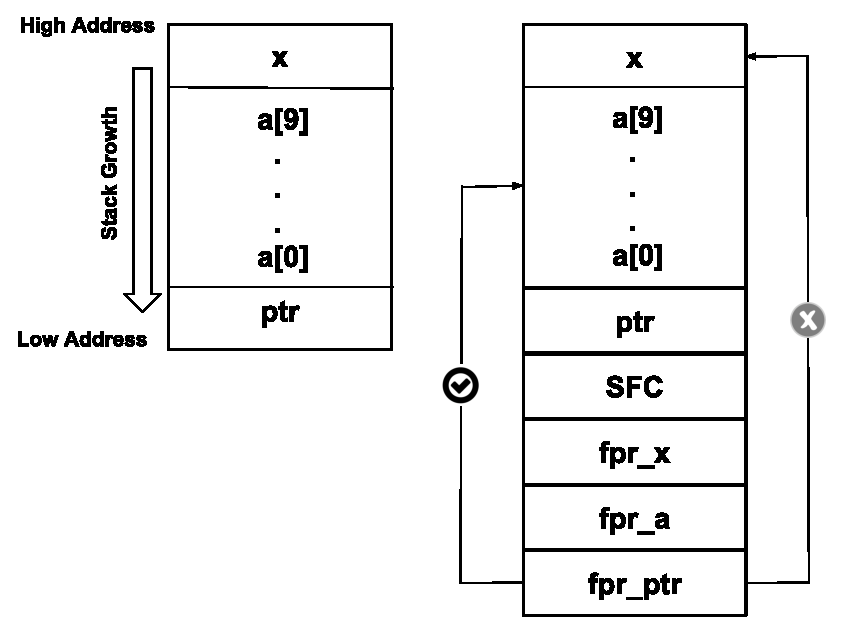
\includegraphics[width=8cm]{stackframe.eps}
\caption{Stack layout with and without fat pointers}
\label{fig:stackframe}
\hrulefill
\end{figure}

Figure \ref{fig:stackframe} clearly describes the difference between the original stack frame and the modified stack frame. We can clearly see that there are fat pointer created for every objects on stacks and placed below the SFC. Now these fat pointers have their own base and bounds(as per Fig \ref{fig: metadata}) and every pointer dereference are first checked for validity and then performed. So the pointer ptr, modified to fpr\_ptr can only access (ptr + 5) and fails to access (ptr + 10).

\section{Architecture and Implementation of \ref{name}}
In the previous section we have discussed our approach to prevent against both spatial and temporal attacks on stacks and heaps. However in this section we would look much deeper into program instrumentation's and implementation aspects of \ref{name}. 

There are many approaches for instrumenting a given piece of code. A said piece of code can be instrumented in the binary level, source level, compiler level or it may have some hardware assistance for code instrumentation. Binary level code instrumentation works to modify the source code after the code is compiled. In this approach instrumentation of the code might require static binary rewriting or partial code emulation at the instruction level where as source level transformation works on the source code to generate an instrumented code which is independent of the instruction set architecture or the C-compiler. But both these binary level instrumentation or the source level transformation suffers from the drawback of efficient compiler level optimisations as the former is applied after the code is compiled and the later being applied before the code is compiled. So in either cases compiler level optimisations might not work properly or it's difficult to implement these compiler level optimisations. Hence in our said approach we choose to work on compiler based instrumentation with hardware assistance for performing the run-time checks. The section below describes the detailed compiler and hardware implementation of \ref{name}.
\subsection{Compiler based Instrumentation}
The compiler based instrumentation needed in \ref{name} is implemented using the RISCV-LLVM compiler infrastructure. LLVM refers to the low level virtual machine which helps to represent the C-code in the intermediate representation(IR) and then allow to perform certain changes in the IR level to generate a modified IR without our concerns for code generation in the back end. To ensure spatial and temporal safety from the compiler perspective we wrote certain analysis passes to analyze some programs and understand the program behaviour. Then we wrote a transformation pass to transform the IR to insert certain compile time checks. The IR transformation pass is divided into multiple steps as described below : 
\begin{figure}
\centering
\captionsetup{justification=centering}
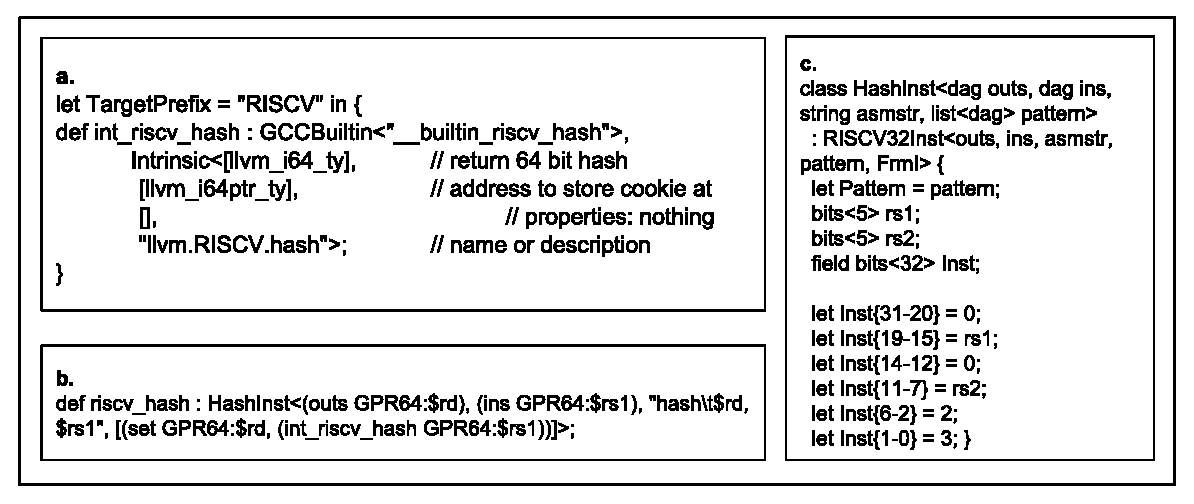
\includegraphics[width=8cm]{intrinsics.eps}
\caption{Code for adding "hash" intrinsic in RISCV-LLVM}
\label{fig:intrinsics}
\hrulefill
\end{figure}

\begin{enumerate}
    \item \textbf{Adding new Instruction Support in LLVM [reference to add new instruction page]} : In our solution we have added two new instruction support namely \textbf{"hash"} and \textbf{"val"} in RISCV-LLVM with the help of intrinsics. These intrinsics are referred as function calls in the LLVM-IR level but eventually will be transformed into instructions in the assembly level.As per LLVM's documentation adding an instruction directly changes the bit code format and it takes a considerable amount of effort to maintain compatibility with the previous versions. So we have proceeded with the concept for adding and intrinsic instead of an instruction. To add a new intrinsic we need to follow the following steps below.\\
    \begin{itemize}
        \item Update \textbf{"Intrinsics.td"} file in "include/llvm/IR/" (Fig.\ref{fig:intrinsics}a).  Here we should declare the intrinsic prototype by giving its name, return type, parameter type and number of parameters it should accept and so on. We should also define the target for the intrinsic i.e. x86 or RISCV, etc. \\
        
        \item Update \textbf{"*InstrInfo.td"} file in "lib/Target/*/"(Fig.\ref{fig:intrinsics}b) (here * implies the target for which you want to generate the assembly code which is RISCV in our case) to give the definition of the intrinsic that we want to generate. It also specifies how our instruction would appear in the assembly code.
        \begin{lstlisting}[language=C]
For eg: hash rd rs1
        \end{lstlisting}
        Here \textbf{"hash"} is the intrinsic that we have added and \textbf{"rs1"} implies the parameter for hash will be present in the rs1 register and the output of this operation will be placed back in the \textbf{"rd"} register.\\
        
        \item Update \textbf{"*InstrFormats.td"} file in "lib/Target/*/"(Fig.\ref{fig:intrinsics}c) (here * implies the code generation target) to provide support for assembly code generation. \\
        
    \end{itemize}
    Fig.\ref{fig:intrinsics} shows the code required to add an intrinsic in RISCV-LLVM\\
    
    \item \textbf{Handling Global variables and structs} : This part of the transformation pass deals with handling global variables, structs and global pointers which might cause a potential threat. Since these variables do not reside in the stack so we cannot directly craft a fat pointer using the SFC. These variables lie in the read only section of the memory known as \textbf{.bss}. To prevent any global pointers to overflow or over read these objects we have crafted fat pointers using the RODC instead. Hence to prevent overflows in the .bss section of memory we used the RODC instead of the SFC.\\
    
    \item \textbf{Replacing malloc calls and free calls with safemalloc and safefree} : This part of the transformation pass replaces all malloc calls with safemalloc and free with safefree and so on.\\
    
    \item \textbf{Adding the stack frame cookie} : This transformation pass adds the SFC for every function calls below all the variables in their own stack frame. It is used to create fat pointer for variables on stack. The transformation also randomizes the SFC before the function exits. This ensures that once the function goes out of scope no pointers of that stack frame can be used to cause any potential threat. \\
    
    \item \textbf{Handling function calls with pointers within the module and outside the module} : This part of the pass takes care of function calls within the module and converts every pointer to fat pointers. However system calls like scanf, printf or function calls outside the module are left untouched. Moreover to protect overflows caused due to special library functions like memcpy and strcpy explicit checks are added to ensure destination buffer length is greater than source buffer length.  \\
    
    \item \textbf{Handling different instruction support in LLVM : } This is the most important part of the transformation pass converting all left over pointers to fat pointers and handling type mismatch of all instructions .It is also responsible for adding all validate checks before every loads and stores. This ensures that whenever a pointer is de-referenced the validate checks must be present. The validate checks are only inserted by the compiler with the help of the "val" instruction but the actual check is performed by the hardware.
\end{enumerate}


\subsection{ISA Extension} \label{ISA} In this section we look into the details of the two new instructions that are inserted by the compiler. 
\begin{enumerate} 
    \item "hash" Instruction \label{hash}: The "hash" instruction is used to compute the \textbf{id\_hash} field the fat pointer. The instruction receives the base address of the SFC for stacks, or base address of the RODC for global variables, or it receives the base addtess of the allocated chunk in case of heaps and returns a 32-bit hash of the value stored in it. The instruction is in the form of 
            \begin{lstlisting}[language=C]
hash rd rs1
        \end{lstlisting}
    where the base address resides in rs1 register and the computed hash value is stored back in rd register.The instruction computes
    \begin{lstlisting}[language=C]
id_hash = hash(*base)
    \end{lstlisting}
    
    \item "val" Instruction \label{val}: The "val" instruction is used to validate the fat pointer. It takes in two arguments the lower 64-bit of the fat pointer and the higher 64-bit of the fat pointer and perform certain validity checks over it. The val instruction is of the form 
            \begin{lstlisting}[language=C]
val rd rs1
        \end{lstlisting}
    where rd represents the higher 64-bit and rs1 represents the lower 64-bit. The val instruction performs certain checks like : 
    \begin{lstlisting}[language=C]
if(BASE==NULL) 
    abort();
if(ID_HASH!=hash(*BASE))
    abort();
if(PTR < BASE || PTR => BOUND)
    abort();
\end{lstlisting}

Here the first two validity checks ensures temporal safety making sure that id\_hash stored along with the fat pointer and hash computed from value stored in base are the same. The third check complies with the spatial safety check ensuring every pointer access is within the base and bound preventing any sort of overflows or over reads. 

\end{enumerate}
\subsection{Micro Architecture}
The hardware and ISA extensions proposed for \ref{name} have been implemented over an existing baseline processor in order to provide a fair comparison of the incurred area and performance overheads.  We have used the 64-bit 5-stage in-order Shakti C-64 design \cite{Shakti} as our baseline processor whose micro-architecture is shown in Figure \ref{} (non-colored blocks refer to the design of the baseline processor). Following  is  a  brief  outline  on  the  functioning  of Shakti C-64:

\begin{enumerate}
    \item \textbf{Fetch Stage} : This  stage  generates  a  new  Program Counter (PC) and fetches the relevant instruction from the Instruction cache (I-cache).  The fetched instruction is then stored in the IF-ID Inter-Stage Buffer (ISB).
    
    \item \textbf{Decode Stage} : This stage reads the instruction from the IF-ID ISB, decodes it to identify the type of instruction, the operand register addresses, the destination register address, etc.  and stores this information in the ID-EXE ISB.
    
    \item \textbf{Execute Stage} : This stage fetches the operands from the register-file and executes the instruction using the ALU (Arithmetic-Logic Unit).  If the instruction is a branch instruction which generates a jump (i.e.  branch is taken) then the IF-ID ISB is invalidated and the PC is set to the new address of the branch.  In case of a memory instruction, this stage  simply  calculates  the  address  of  the  memory  access. The result of the execution is stored in the EXE-MEM ISB.
    
    \item \textbf{Memory Stage} : If the instruction executed does not require access to the memory/cache then it is simply buffered into  MEM-WB  ISB.  However,  in  case  of  a  load/  store instruction the request is sent to the data cache to perform the  necessary  operation.   On  completion  of  the  memory/cache access, the information is stored in the MEM-WB ISB.
    
    \item \textbf{Write Back} : This is the final stage of the processor  which  commits  the  result  into  the  register-file  if  no exception was generated for that instruction in any of the previous  stages.   In  case  a  trap  is  generated,  all  the  ISBs are invalidated and the PC in the fetch stage is set to the address of the specific Interrupt Service Routine (ISR).
    
    need to write more about how the two new instructions work in the hardware. also need to add an image like shakti-t paper of the low level architecture.
\end{enumerate}

\section{Case Study}

In this section we would look into detailed LLVM-IR code of different parts of a simple C-program and see how the transformation pass modifies the said code and generate the modified LLVM-IR. The transformation pass is implemented in RISCV-LLVM version ...and hence the code lowering will
be done according to the RISCV architecture. Given below are some of the examples of the basic transformation pass.

\begin{enumerate}
    \item \textbf{Handling the SFC } : Given below is the LLVM IR code to insert the SFC and collapse it just before the function exits. The keyword \textbf{"alloca"}is used to allocate a memory on the stack and all variables with '\%' sign represent a temporary register. LLVM uses the concept of static single assignment and has infinite no of registers for computation purposes.  
    \begin{lstlisting}[language=LLVM]
//insert this at the end of all variables
%stack_cookie = alloca i64
%2 = call i64 @random64()
store i64 %2, i64* %stack_cookie
//body of the function call
...
//insert this at the end of the function
%4 = call i64 @random64()
store i64 %4, i64* %stack_cookie
%stack_cookie_burn = call 
i64 @llvm.RISCV.hash(i64* %stack_cookie)
\end{lstlisting}
    Here "@llvm.RISCV.hash" represents the intrinsic call to our function hash.
    
    \item \textbf{Crafting fat pointers} : Crafting a fat pointer is done by calling a method craft with four parameters namely base, bound, id\_hash and the pointer itself. The craft function is a few lines assembly code  inserted during code lowering. The craft function below is used to craft a fat pointer for a character array of size 10. 
    \begin{lstlisting}[language=LLVM]
...
%stack_cookie_32 = ptrtoint i64* %stack_cookie 
to i32
...
%stack_hash = trunc i64 %stack_hash_long 
to i32
%2 = alloca [10 x i8], align 1
%pti1 = ptrtoint [10 x i8]* %2 to i32
%absolute_bnd2 = add i32 %pti1, 10
%fpr3 = call i128 @craft(i32 %pti1, 
i32 %stack_cookie_32, i32 %absolute_bnd2,
i32 %stack_hash)

    \end{lstlisting}
    
    \item \textbf{Validating Loads and Stores} : As stated earlier every loads and stores are validated. Let us take a single line of C code and see how the following code gets transformed by adding validity checks before every loads and store.
    \begin{lstlisting}[language=C]
a[5] = *(ptr+3);
    \end{lstlisting}
    Here 'a' is an array of size 10 and ptr is a pointer pointing to the array. The code below is the LLVM IR representation of the said line:
    \begin{lstlisting}[language=C]
%2 = alloca [10 x i8], align 1
%3 = alloca i8*, align 8
%6 = load i8*, i8** %3, align 8
%7 = getelementptr inbounds i8, i8* %6, i64 3
%8 = load i8, i8* %7, align 1

%9 = getelementptr inbounds [10 x i8], 
[10 x i8]* %2, i64 0, i64 5
store i8 %8, i8* %9, align 1
    \end{lstlisting}
    Assuming the fat pointers exists for the variables the different instructions get modified as follows : 
    \begin{lstlisting}
...
%fpr3 = call i128 @craft(...)
...
%fpr6 = call i128 @craft(...)

%fpr_low13 = trunc i128 %fpr6 to i64
%fpr_hi_big14 = lshr i128 %fpr6, 64
%fpr_hi15 = trunc i128 %fpr_hi_big14 to i64
call void @llvm.RISCV.validate(i64 %fpr_hi15,
i64 %fpr_low13)
%ptr32_16 = and i64 %fpr_low13, 4294967295
%ptrl = inttoptr i64 %ptr32_16 to i128*
%fpld = load i128, i128* %ptrl, align 8

%zextarrayidx17 = zext i32 3 to i128
%arrayidx18 = add i128 %fpld, %zextarrayidx17
;validate arrayidx18
...
%ptrl23 = inttoptr i64 %ptr32_22 to i8*
%5 = load i8, i8* %ptrl23, align 1
%zextarrayidx24 = zext i32 5 to i128
%arrayidx25 = add i128 %fpr3, 
;validate arrayidx25
...
%ptrs30 = inttoptr i64 %ptr32_29 to i8*
store i8 %5, i8* %ptrs30, align 1

    \end{lstlisting}
    The above code also shows that all the "getelementptr" instructions has been transformed to offsets and added with the fatpointers to point to the desired location of memory.\\
    
    \item \textbf{Handling external function calls like strcpy} : To handle external function calls like strcpy explicits check for length of the destination and source buffer needs to be performed. This is because we do not have any control of the external function and these can cause overflows of buffer. Let us look at the sample code below : 
     \begin{lstlisting}[language=C]
char a[10],b[10];
...
strcpy(a,b);
     \end{lstlisting}
     The LLVM representation of the following code is given below assuming that the arrays have their respective allocations and so on: 
     \begin{lstlisting}[language=LLVM]
...
%5 = getelementptr inbounds [10 x i8],
[10 x i8]* %2, i32 0, i32 0
%6 = getelementptr inbounds [10 x i8],
[10 x i8]* %3, i32 0, i32 0
%7 = call i8* @strcpy(i8* %5, i8* %6)
     \end{lstlisting}
     The modified LLVM-IR code is  : 
     \begin{lstlisting}[language=LLVM]
...
%zextarrayidx = zext i32 0 to i128
%arrayidx = add i128 %fpr3, %zextarrayidx
%zextarrayidx8 = zext i32 0 to i128
%arrayidx9 = add i128 %fpr6, %zextarrayidx8
%fpr_low10 = trunc i128 %arrayidx to i32
%ptrc11 = inttoptr i32 %fpr_low10 to i8*
%fpr_low12 = trunc i128 %arrayidx9 to i32
%ptrc13 = inttoptr i32 %fpr_low12 to i8*
%source_len = call i64 @strlen(i8* %ptrc13)
%check_len = icmp ule i64 10, %source_len
br i1 %check_len, label %5, label %7
...
     \end{lstlisting}
   In the above modified code if the condition of the branch instruction is true then the code jumps to a basic block and finally exits else normal execution is followed\\.   
    
    \item \textbf{Malloc} : In LLVM IR the malloc call would get transformed into a safemalloc call. Let us look at a simple example of how the original IR looks and the modified IR is generated. 
     \begin{lstlisting}[language=C]
char *q = malloc(10);
     \end{lstlisting}
     
     The corresponding LLV IR code would look something like this:
     \begin{lstlisting}[language=LLVM]
%1 = alloca i8*, align 8
%2 = call i8* @malloc(i64 zeroext 10)
store i8* %2, i8** %1, align 8
     \end{lstlisting}
where \%1 refers to the allocation of variable 'q' and then allocating a size of 10 bytes and then allocating the size back to q. The modified IR code is given below : 
    \begin{lstlisting}[language=LLVM]
%1 = alloca i128, align 8
...
%fpr = call i128 @craft(i32 %pti, 
i32 %stack_cookie_32, i32 %absolute_bnd,
i32 %stack_hash)
%3 = call i128 @safemalloc(i64 zeroext 10)
;validate and store
...
call void @llvm.RISCV.validate(i64 
%fpr_hi, i64 %fpr_low)
...
store i128 %3, i128* %ptrs, align 8

     \end{lstlisting}
     
    \item \textbf{Free} : Similar to the malloc call the free call also gets modified into safefree and it now accepts a 128-bit fat pointer instead of a normal pointer. Let us take a sample code of free and see how the transformation pass works.
    \begin{lstlisting}[language=C]
free(q);
     \end{lstlisting}
     
     Assuming that the above malloc code was in place now the free call to q would look like something like :
     \begin{lstlisting}[language=LLVM]
%3 = load i8*, i8** %1, align 8
call void @free(i8* %3)
     \end{lstlisting}
    where \%1 represents the same variable shown in the malloc code above. The modified LLVM code is given below : 
    \begin{lstlisting}[language=LLVM]
;validate and load
...
call void @llvm.RISCV.validate(i64 %fpr_hi3,
i64 %fpr_low1)
...
%fpld = load i128, i128* %ptrl, align 8
call void @safefree(i128 %fpld)

     \end{lstlisting}
\end{enumerate}

\section{Results}
The \ref{name} micro-architecture has been developed using Bluespec-System-Verilog ... write something more here. The results for performance overhead and effectiveness are both observed in a simulation environment and the hardware developed, in order to match the correctness of the hardware. To run the programs on a simulation environment we have used spike along with proxy kernel over a 1.6Ghz Intel Core i7 processor with 16GB ram. Moreover to calculate the cycle count in the simulation environment we have added two assembly instructions ("rdcycle" instruction of RISCV) in the C-code.


\begin{figure*}[h]
\centering
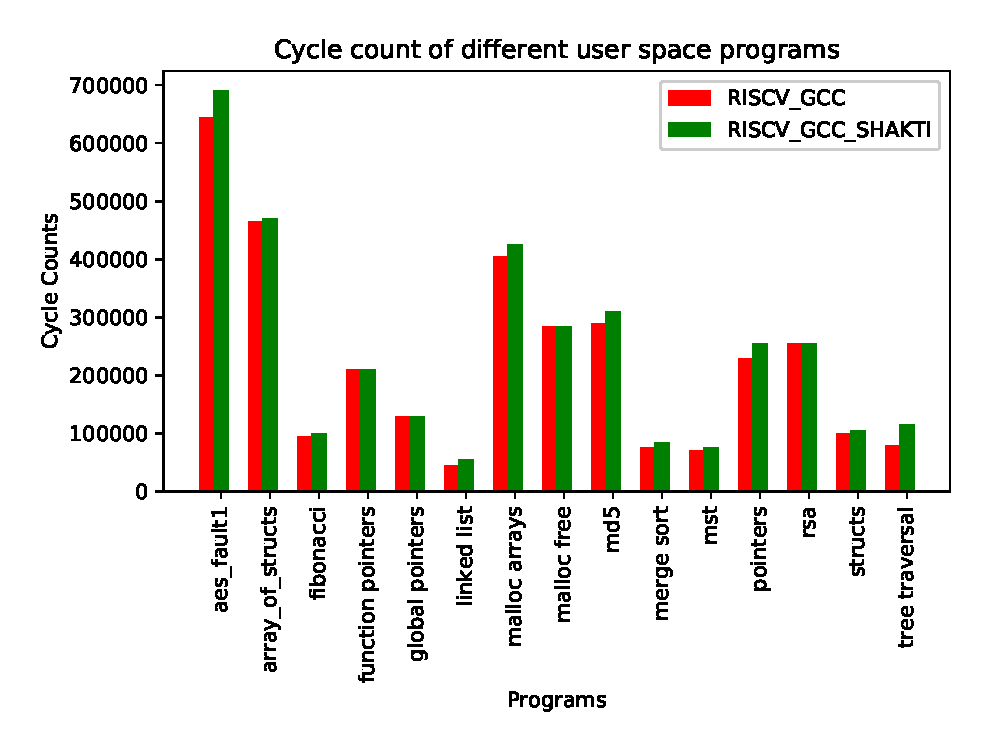
\includegraphics[scale=0.75]{overheads.eps}
\caption{\scshape{Graph demonstrating cycle count overheads of different user space programs. }}\label{fig:overhead}
\end{figure*} 

\subsection{Calculating Runtime Overheads : }

\subsection{Effectiveness : } To check the effectiveness of bounds checking and use after free attacks we have used the SARD-dataset-81 and SARD-dataset-89 download from SAMATE-NIST\cite{SARD} website. The dataset had around 1100 programs consisting of both good and vulnerable ones and our approach were able to detect almost all of the vulnerable programs with some false negatives. The issues relating to false negatives were some of the multi-threading programs and nested sub-object protection that are yet to be handled. Sub-object protection is handled to ensure that it does not overflow the object itself but tighter bound to protect sub-objects were omitted to reduce the incurred overhead. Moreover it did not had any issues pertaining to false positives.

\subsection{Running user space programs : }
To test the hardware developed by our team, we have written some user space programs of different types ranging from stack overflows to heap overflows, testing arrays of structs, function pointers, linked list and so on. The results were compared by running these programs in simulation mode and on the hardware developed. We used "spike" which is a RISCV simulator to run these test programs along with proxy kernel to support the external library calls. To ensure proper mimicking of the hardware we had to add instruction supports for "hash" and "val" in spike as well. In the simulation environment these programs had a cycle count overhead of less than 9\%.

Figure \ref{fig:overhead} shows the cycle count overhead for some of the programs 

\section{Conclusion}

% \subsection{Math Equations}
% You may want to display math equations in three distinct styles:
% inline, numbered or non-numbered display.  Each of
% the three are discussed in the next sections.

% \subsubsection{Inline (In-text) Equations}
% A formula that appears in the running text is called an
% inline or in-text formula.  It is produced by the
% \textbf{math} environment, which can be
% invoked with the usual \texttt{{\char'134}begin\,\ldots{\char'134}end}
% construction or with the short form \texttt{\$\,\ldots\$}. You
% can use any of the symbols and structures,
% from $\alpha$ to $\omega$, available in
% \LaTeX~\cite{Lamport:LaTeX}; this section will simply show a
% few examples of in-text equations in context. Notice how
% this equation:
% \begin{math}
%   \lim_{n\rightarrow \infty}x=0
% \end{math},
% set here in in-line math style, looks slightly different when
% set in display style.  (See next section).

% \subsubsection{Display Equations}
% A numbered display equation---one set off by vertical space from the
% text and centered horizontally---is produced by the \textbf{equation}
% environment. An unnumbered display equation is produced by the
% \textbf{displaymath} environment.

% Again, in either environment, you can use any of the symbols
% and structures available in \LaTeX\@; this section will just
% give a couple of examples of display equations in context.
% First, consider the equation, shown as an inline equation above:
% \begin{equation}
%   \lim_{n\rightarrow \infty}x=0
% \end{equation}
% Notice how it is formatted somewhat differently in
% the \textbf{displaymath}
% environment.  Now, we'll enter an unnumbered equation:
% \begin{displaymath}
%   \sum_{i=0}^{\infty} x + 1
% \end{displaymath}
% and follow it with another numbered equation:
% \begin{equation}
%   \sum_{i=0}^{\infty}x_i=\int_{0}^{\pi+2} f
% \end{equation}
% just to demonstrate \LaTeX's able handling of numbering.

% \subsection{Citations}
% Citations to articles~\cite{bowman:reasoning,
% clark:pct, braams:babel, herlihy:methodology},
% conference proceedings~\cite{clark:pct} or maybe
% books \cite{Lamport:LaTeX, salas:calculus} listed
% in the Bibliography section of your
% article will occur throughout the text of your article.
% You should use BibTeX to automatically produce this bibliography;
% you simply need to insert one of several citation commands with
% a key of the item cited in the proper location in
% the \texttt{.tex} file~\cite{Lamport:LaTeX}.
% The key is a short reference you invent to uniquely
% identify each work; in this sample document, the key is
% the first author's surname and a
% word from the title.  This identifying key is included
% with each item in the \texttt{.bib} file for your article.

% The details of the construction of the \texttt{.bib} file
% are beyond the scope of this sample document, but more
% information can be found in the \textit{Author's Guide},
% and exhaustive details in the \textit{\LaTeX\ User's
% Guide} by Lamport~\shortcite{Lamport:LaTeX}.

% This article shows only the plainest form
% of the citation command, using \texttt{{\char'134}cite}.

% Some examples.  A paginated journal article \cite{Abril07}, an enumerated
% journal article \cite{Cohen07}, a reference to an entire issue \cite{JCohen96},
% a monograph (whole book) \cite{Kosiur01}, a monograph/whole book in a series (see 2a in spec. document)
% \cite{Harel79}, a divisible-book such as an anthology or compilation \cite{Editor00}
% followed by the same example, however we only output the series if the volume number is given
% \cite{Editor00a} (so Editor00a's series should NOT be present since it has no vol. no.),
% a chapter in a divisible book \cite{Spector90}, a chapter in a divisible book
% in a series \cite{Douglass98}, a multi-volume work as book \cite{Knuth97},
% an article in a proceedings (of a conference, symposium, workshop for example)
% (paginated proceedings article) \cite{Andler79}, a proceedings article
% with all possible elements \cite{Smith10}, an example of an enumerated
% proceedings article \cite{VanGundy07},
% an informally published work \cite{Harel78}, a doctoral dissertation \cite{Clarkson85},
% a master's thesis: \cite{anisi03}, an online document / world wide web
% resource \cite{Thornburg01, Ablamowicz07, Poker06}, a video game (Case 1) \cite{Obama08} and (Case 2) \cite{Novak03}
% and \cite{Lee05} and (Case 3) a patent \cite{JoeScientist001},
% work accepted for publication \cite{rous08}, 'YYYYb'-test for prolific author
% \cite{SaeediMEJ10} and \cite{SaeediJETC10}. Other cites might contain
% 'duplicate' DOI and URLs (some SIAM articles) \cite{Kirschmer:2010:AEI:1958016.1958018}.
% Boris / Barbara Beeton: multi-volume works as books
% \cite{MR781536} and \cite{MR781537}.

% A couple of citations with DOIs: \cite{2004:ITE:1009386.1010128,
%   Kirschmer:2010:AEI:1958016.1958018}.

% Online citations: \cite{TUGInstmem, Thornburg01, CTANacmart}.


% \subsection{Tables}
% Because tables cannot be split across pages, the best
% placement for them is typically the top of the page
% nearest their initial cite.  To
% ensure this proper ``floating'' placement of tables, use the
% environment \textbf{table} to enclose the table's contents and
% the table caption.  The contents of the table itself must go
% in the \textbf{tabular} environment, to
% be aligned properly in rows and columns, with the desired
% horizontal and vertical rules.  Again, detailed instructions
% on \textbf{tabular} material
% are found in the \textit{\LaTeX\ User's Guide}.

% Immediately following this sentence is the point at which
% Table~\ref{tab:freq} is included in the input file; compare the
% placement of the table here with the table in the printed
% output of this document.

% \begin{table}
%   \caption{Frequency of Special Characters}
%   \label{tab:freq}
%   \begin{tabular}{ccl}
%     \toprule
%     Non-English or Math&Frequency&Comments\\
%     \midrule
%     \O & 1 in 1,000& For Swedish names\\
%     $\pi$ & 1 in 5& Common in math\\
%     \$ & 4 in 5 & Used in business\\
%     $\Psi^2_1$ & 1 in 40,000& Unexplained usage\\
%   \bottomrule
% \end{tabular}
% \end{table}

% To set a wider table, which takes up the whole width of the page's
% live area, use the environment \textbf{table*} to enclose the table's
% contents and the table caption.  As with a single-column table, this
% wide table will ``float'' to a location deemed more desirable.
% Immediately following this sentence is the point at which
% Table~\ref{tab:commands} is included in the input file; again, it is
% instructive to compare the placement of the table here with the table
% in the printed output of this document.


% \begin{table*}
%   \caption{Some Typical Commands}
%   \label{tab:commands}
%   \begin{tabular}{ccl}
%     \toprule
%     Command &A Number & Comments\\
%     \midrule
%     \texttt{{\char'134}author} & 100& Author \\
%     \texttt{{\char'134}table}& 300 & For tables\\
%     \texttt{{\char'134}table*}& 400& For wider tables\\
%     \bottomrule
%   \end{tabular}
% \end{table*}
% % end the environment with {table*}, NOTE not {table}!

% It is strongly recommended to use the package booktabs~\cite{Fear05}
% and follow its main principles of typography with respect to tables:
% \begin{enumerate}
% \item Never, ever use vertical rules.
% \item Never use double rules.
% \end{enumerate}
% It is also a good idea not to overuse horizontal rules.


% \subsection{Figures}

% Like tables, figures cannot be split across pages; the best placement
% for them is typically the top or the bottom of the page nearest their
% initial cite.  To ensure this proper ``floating'' placement of
% figures, use the environment \textbf{figure} to enclose the figure and
% its caption.

% This sample document contains examples of \texttt{.eps} files to be
% displayable with \LaTeX.  If you work with pdf\LaTeX, use files in the
% \texttt{.pdf} format.  Note that most modern \TeX\ systems will convert
% \texttt{.eps} to \texttt{.pdf} for you on the fly.  More details on
% each of these are found in the \textit{Author's Guide}.

% \begin{figure}
% %\includegraphics{fly}\Description{A fly}
% \caption{A sample black and white graphic.}
% \end{figure}

% \begin{figure}
% %\includegraphics[height=1in, width=1in]{fly}\Description{A fly image,
% %  to $1''\times1''$}
% \caption{A sample black and white graphic
% that has been resized with the \texttt{includegraphics} command.}
% \end{figure}


% As was the case with tables, you may want a figure that spans two
% columns.  To do this, and still to ensure proper ``floating''
% placement of tables, use the environment \textbf{figure*} to enclose
% the figure and its caption.  And don't forget to end the environment
% with \textbf{figure*}, not \textbf{figure}!

% \begin{figure*}
% %\includegraphics{flies}\Description{Several flies, spanning two
% %  columns of text}
% \caption{A sample black and white graphic
% that needs to span two columns of text.}
% \end{figure*}


% \begin{figure}
% %\includegraphics[height=1in, width=1in]{rosette}\Description{A %rosette}
% \caption{A sample black and white graphic that has
% been resized with the \texttt{includegraphics} command.}
% \end{figure}